\chapter{基于深度学习的意图识别与语义槽填充方法}

\section{语义理解问题描述}
跨界服务平台内服务的智能调用实现过程中,接受的是用户输入的一句有目的性的话,系统在语义理解的过程中,首先要识别用户的意图,对应到系统就是根据
用户意图匹配相应的服务以及匹配该服务要执行的操作,这两者均可被视为分类问题,可以用深度学习的分类算法解决;找到匹配的服务以后,在服务执行前需要
必要的执行参数,可以从用户输入的语句中提取,这将被看作语义槽填充问题,可以用序列标注算法解决。
在本系统中,服务,意图,语义槽(即服务参数)三者具有强相关的关系,

以调用航班信息查询服务为例,来解释跨界服务平台内服务,意图,语义槽(即服务参数)。用户在进入跨界服务平台后,输入“查询成都飞往杭州的航班”,跨界服务平台内
的语义理解模型识别出该语义对应平台内部的<flight机票航班服务>,用户意图为<query查询>,语义槽(即服务参数)为<startCity起始地>成都和<endCity目的地>杭州


\begin{figure}[htbp]
    \centering
    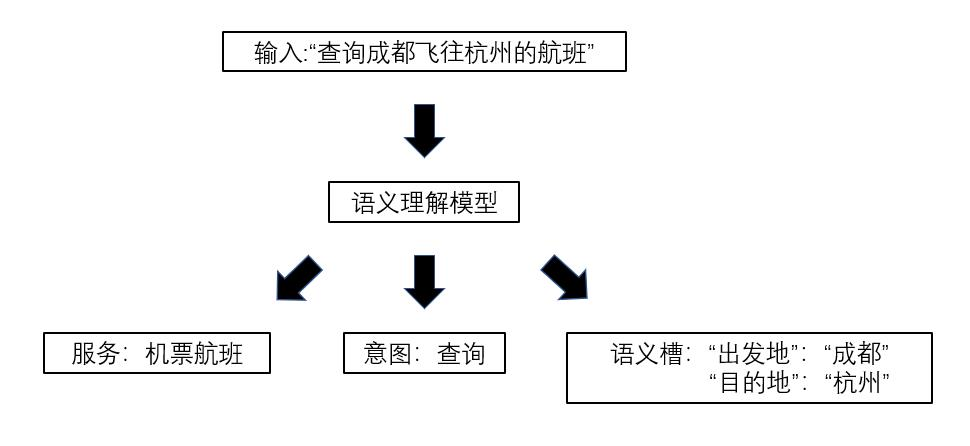
\includegraphics[scale=0.5]{./images/questiondesc.jpg}
    \caption{系统语义理解示例}
    \label{fig:questiondesc}
  \end{figure}


\section{文本预处理}
\subsection{文本分词}
用户不需要输入完整的句子

\subsection{标签的结构化表示}

\section{算法流程整体描述}

\section{服务分类模型}
LSTM是一种特殊的RNN,能够学习长期依赖关系,擅长处理文本序列的问题;CNN多用于图像领域,由于卷积核的存在,能够提取出词与词之间的隐藏的语义信息,本文将他应用到nlp领域。
因此本节将两者结合,提出CNN-LSTM模型用以解决服务分类问题。

\begin{figure}[htbp]
    \centering
    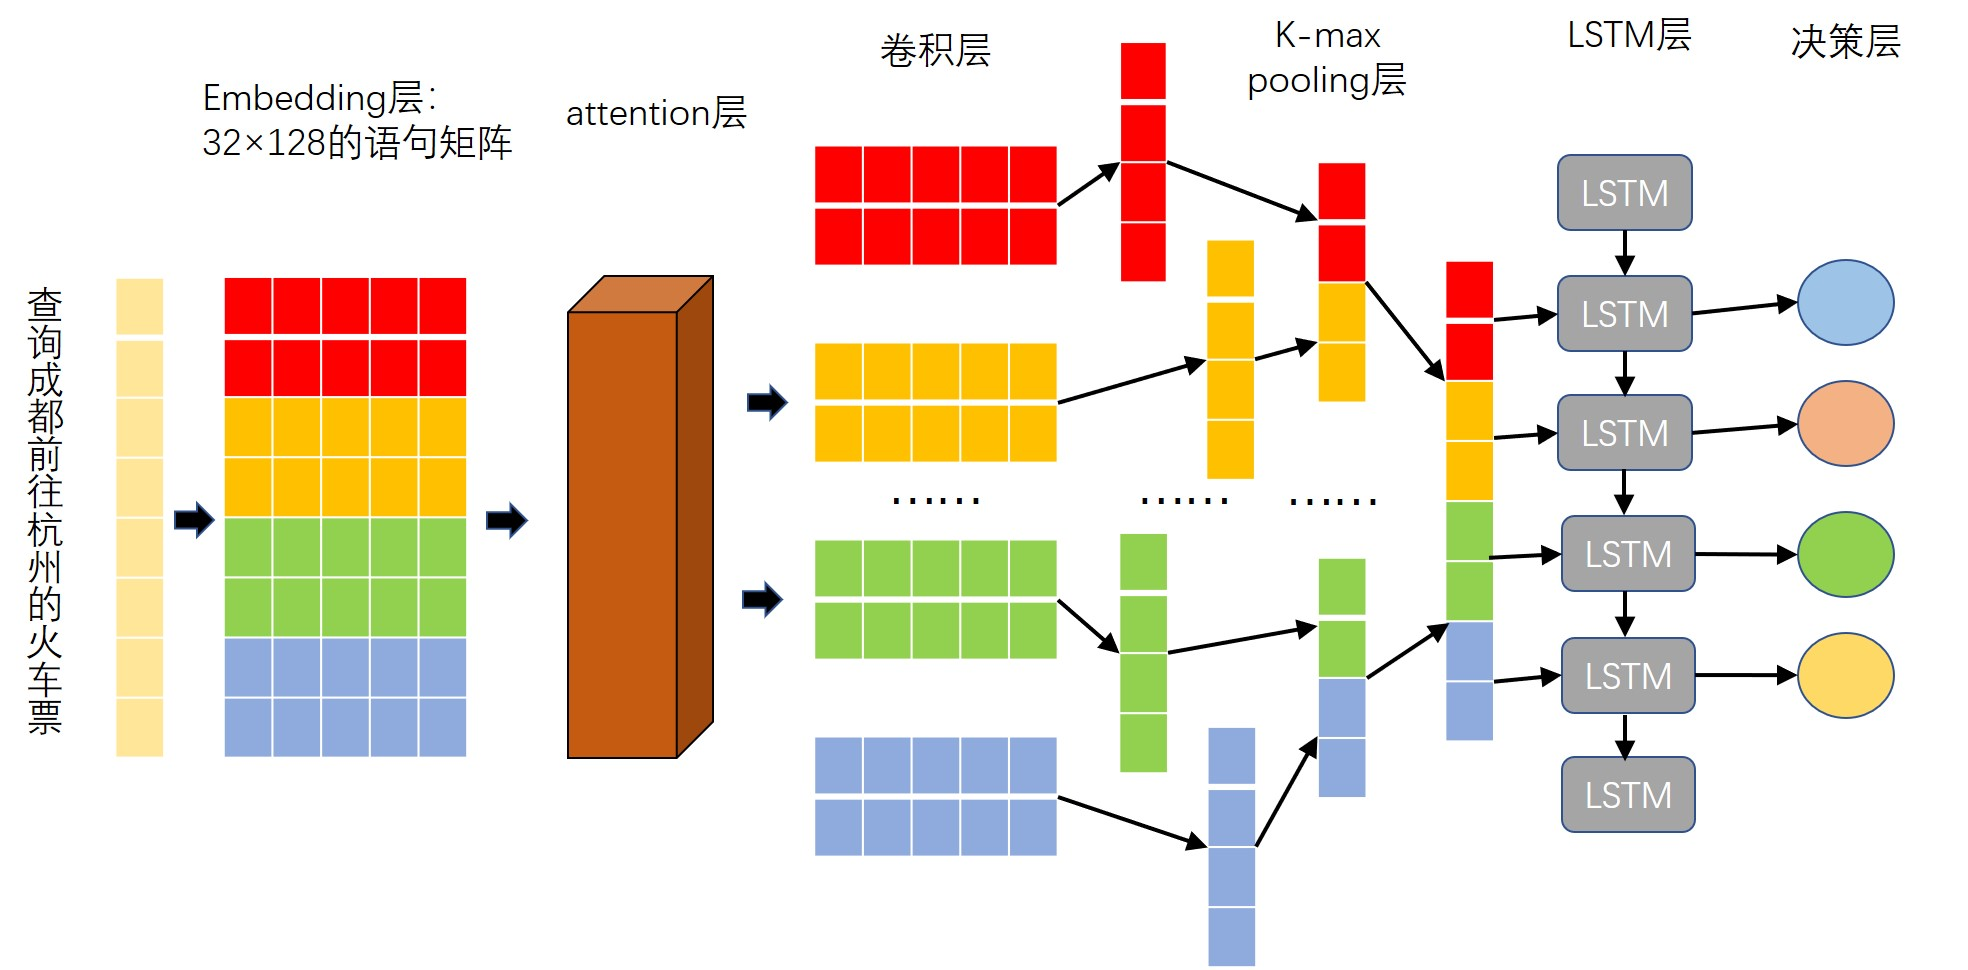
\includegraphics[scale=0.5]{./images/cnn-lstm.jpg}
    \caption{服务分类模型}
    \label{fig:cnn-lstm}
  \end{figure}








